%!TEX root = main.tex
\documentclass[a4paper,12pt]{report}

% The packages are useful for many mathematical symbols but you may well not need them
\usepackage{amsmath,amssymb,amscd}
\usepackage{paralist}
\usepackage{bookmark}

\usepackage{caption}
% \usepackage{subcaption}
\usepackage[justification=RaggedRight,
            format=hang]{subcaption}

\usepackage{hyperref}
\usepackage[usenames,dvipsnames]{xcolor}
\hypersetup{
  colorlinks = true,
  citecolor  = RoyalBlue,
  linkcolor  = RoyalBlue,
  urlcolor   = RoyalBlue,
}

% \let\subsectionautorefname\sectionautorefname
% \let\subsubsectionautorefname\sectionautorefname

% This is great for reading in images
\usepackage{graphicx}
\usepackage{footnote}
\captionsetup[subfigure]{width=0.9\textwidth}

\usepackage[backend=bibtex,style=authoryear,maxcitenames=2,natbib=true]{biblatex} % Use the bibtex backend with the authoryear citation style (which resembles APA)


\addbibresource{library.bib}

% This is great for drafts as it will show all the labels you have defined.
% DON'T forget to comment it out before submission
%\usepackage{showkeys}

% Change Page Size
\typeout{--- Increasing width and height of text }
% A4 paper is 297mm high and 210mm wide.
\setlength{\textwidth}{16.00cm} % OK for both Letter and A4
\setlength{\oddsidemargin}{-0.04cm}  % actual margins = 1inch + \oddsidemargin
                                 %top/odd/even-sidemargin
\setlength{\evensidemargin}{-0.04cm} %  ditto
\setlength{\topmargin}{-1.0cm}      %  ditto
\setlength{\headheight}{18pt} \setlength{\headsep}{6pt}
\setlength{\topskip}{0pt}  %see pp155 also about baselineskip
\setlength{\textheight}{23.0cm} % 25cm for A4, 23cm for Letter or DJ
\setlength{\footskip}{0.7cm}


\begin{document}

\begin{titlepage}
  \center

  \vspace*{2cm}
  \textsc{\Large Imperial College London}\\[0.5cm] 
  \textsc{\large Department of Physics}\\[0.5cm] 

  \title{\bf{Light bending in general relativity with a cosmological constant: a literature review}}
  \date{4 October, 2017}
  \author{Lingyi Hu\\ CID: \texttt{00919977}}

  {\let\newpage\relax\maketitle}
  \thispagestyle{empty}

  \vspace*{1cm}
  \noindent
  \large
  {\bf Project code:} ASTR-Heavens-1\par
  {\bf Supervisor:} Prof Alan \textsc{Heavens}\par
  {\bf Assessor:} Prof Carlo \textsc{Contaldi}

  \vspace*{1cm}

  {\bf Word count:}
  2478 words (excluding title page and bibliography)
  % 91 + 187 + 837 + 865 + 400 + 198

  \vspace*{2cm}


\end{titlepage}


\vspace*{2cm}
\noindent
{\bf Abstract:} In this review, I survey some of the work analyzing the effect of the cosmological constant on gravitational deflection of light, a debate started mainly in a paper by \citet{Rindler2007} which challenged the conventional opinion. Since then, numerous papers have been written both in support and rebuttal of Rindler and Ishak. I go through the main arguments for and against a $\Lambda$-dependence in the lensing equation, identify limitations of some approaches, and look at the direction in which further work can take to settle this debate. 

% \newpage


%!TEX root = ../thesis.tex
\chapter{Introduction}

There has been a debate over the past decade about whether the cosmological constant enters directly into the gravitational lensing equation. 

The conventional view \cite{islam1983cosmological} states that the cosmological constant does not directly play a role in gravitational lensing, \cite{simpson2010lensing} apart from 
%!TEX root = ../main.tex
\section{Conventional argument using the null geodesic}\label{section:conventional}

We are concerned about whether $\Lambda$ contributes to the bending of light around a concentrated mass. Conventional view, first put forth by \citet{Islam1983}, is that it does not, and classical lensing is correct as it is. This view, supported by multiple authors \citep{Lake2002,Finelli2007,Park2008,Simpson2008}, argues that the equations describing the path followed by a photon, the null geodesic equations, takes the same form with or without $\Lambda$ in the Kottler metric. 

The Kottler metric \citep{Kottler1918} represents the Schwarzschild vacuum metric extended to include a cosmological constant. In terms of curvature coordinates ($r$, $\theta$, $\phi$, $t$), the line element in Kottler space is given by

\begin{equation}
  ds^2 = f(r) dt^2 - \frac{dr^2}{f(r)} - r^2 (d \theta^2 + \sin^2 \theta d \phi^2)
  \label{eq:kottler-metric}
\end{equation} 
where 
\begin{equation}
  f(r) = 1 - \frac{2m}{r} - \frac{\Lambda r^2}{3},
  \label{eq:kottler-metric2}
\end{equation}
and $m$ is the mass of the central object and relativistic units ($C = G = 1$) are used. 

There is general agreement \citep{Lake2002,Rindler2007} that when we consider the null geodesic of such a metric, the cosmological constant drops out of the $r$, $\phi$ second-order differential equation in polar coordinates without approximation, and therefore does not contribute to light bending. \citet{Islam1983} found that the differential equation governing light rays moving in a Kottler metric simplifies to

\begin{equation}
  \frac{d^2 u}{d \phi^2} + u = 3mu^2
  \label{eq:null-geodesic-kottler}
\end{equation}
where $u = 1/r$. This formula is independent of $\Lambda$, therefore the resulting solution to this differential equation is the same as in a pure Schwarzschild background. For years this has been the accepted view, supported by the intuition that the cosmological constant is uniform but gravitational lensing occurs as a result of inhomogeneities in the spacetime. 


\section{$\Lambda$ contribution to light bending in Kottler spacetime}\label{section:kottler}

This official opinion was however challenged by \citet{Rindler2007}, who argue that while the $\Lambda$ term drops out of the null geodesic, $\Lambda$ still affects light bending through the metric itself, since the photon is moving in $\Lambda$-dependent geometry. As space is not asymptotically flat, the process of measurement causes the cosmological constant to creep into the light bending angle. 

As noted by \citet{Gibbons2008}, the confusion with the conventional literature lies mainly in the question of what precisely \eqref{eq:null-geodesic-kottler} represents. \eqref{eq:null-geodesic-kottler} merely governs the projection of null rays onto the spatial sections of the metric, but not the more complex geometrical features. Rindler and Ishak's paper attempt to address this. 

They started with the Kottler metric and noted that due to the spherical symmetry of the spatial part of the metric, any orbit must lie entirely in one of the central spatial equatorial coordinate ``plane'' $\theta = \pi / 2$, and in Kottler spacetime this is given by the 2-metric

\begin{equation}
  dl^2 = \left ( 1 - \frac{2m}{r} - \frac{\Lambda r^2}{3}\right )^{-1} dr^2 + r^2 d \phi^2. 
\end{equation}
Without the $\Lambda$ term, this reduces to the Schwarzschild 2-metric. Near the central mass, where the $2m/r$ term dominates over $\Lambda r^2 / 3$, we get the geometry of the upper half of Flamm Paraboloid \citep{Flamm1916}, which has the equation

\begin{equation}
  z^2 = 8m (r - 2m)
\end{equation}
in cylindrical polar coordinates in ordinary 3D Euclidean space. On the other hand, when the $\Lambda r^2 / 3$ term dominates over $2m/r$, we obtain the geometry of a sphere. The Kottler metric is a combination of the two geometries, and the authors are concerned with the region between these two boundaries. 

\begin{figure}
  \centering
  % 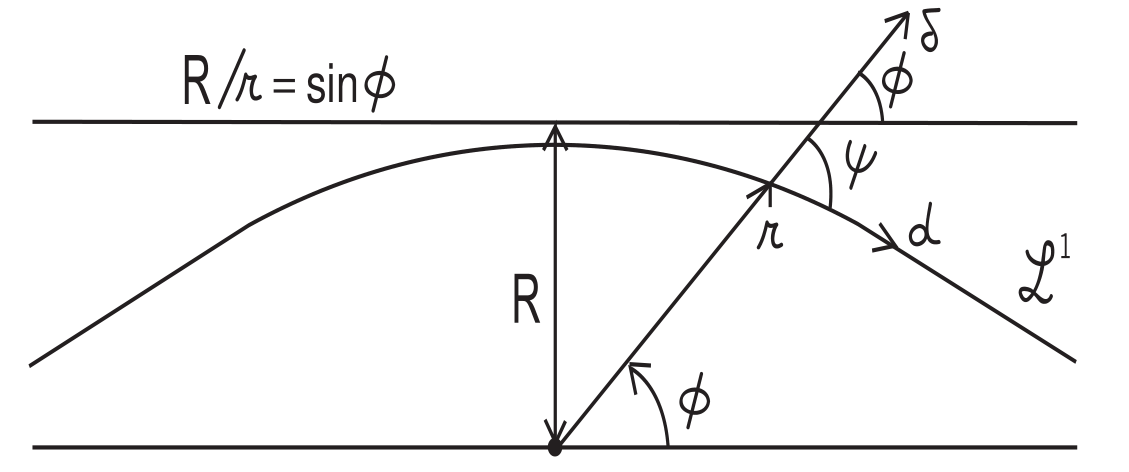
\includegraphics[height=0.5\linewidth]{img/rindler-ishak-2.png}
  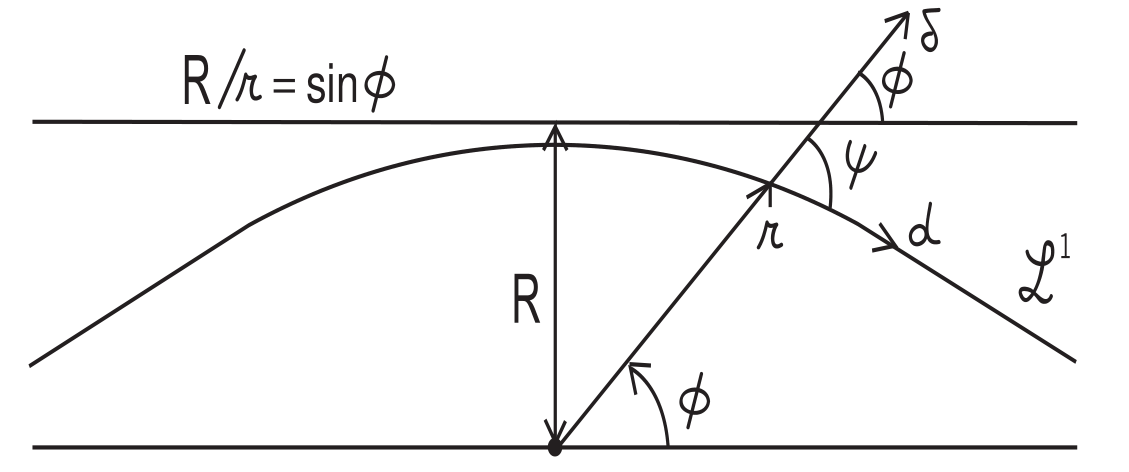
\includegraphics{img/rindler-ishak-2.png}
  \caption{This is the orbital map from \citet{Rindler2007}, describing the plane graph of the orbit equation. The one-sided deflection angle is $\psi - \phi \equiv \epsilon$. }
  \label{fig:rindler-ishak-2}
\end{figure}

Starting with the first approximation of the null geodesic equation \eqref{eq:null-geodesic-kottler}, the authors use the cosine formula for the angle between two coordinate directions

\begin{equation}
  \cos (\psi) = \frac{g_{ij} d^i \delta ^j}{(g_{ij} d^i d^j)^{1/2} (g_{ij} \delta^i \delta^j)^{1/2}}
  \label{eq:cosine-formula}
\end{equation}
to calculate the bending angle $\Psi$ measured by an observer at an arbitrary point $(r, \phi)$ between a ray coming radially from the centre and the ray skirting the lens (see Figure \ref{fig:rindler-ishak-2}). They found that, when the observer and source are equidistant from the lens (i.e. observer is at $\phi = 0$ in Figure \ref{fig:rindler-ishak-2}, arbitrarily chosen), the total light bending angle $\alpha$ to first order in $m / R$ is given by 

\begin{equation}
  \alpha \approx 2 \frac{m}{R} - \frac{\Lambda R^3}{12m}
  \label{eq:rindler-ishak-correction}
\end{equation}
where the first term is simply the classical gravitational lensing bending angle to first order, and the second term is the first order correction to the classical bending angle. 
% As expected from the repulsive nature of $\Lambda$, a positive $\Lambda$ reduces the bending angle. 

The paper by Rindler and Ishak renewed interest in the problem and sparked fresh debate. The authors followed this up with two other papers \citep{Ishak2008b,Ishak2008} that reiterated and elaborated upon their claim. In one of them \citep{Ishak2008b}, they referred to observations of several lensing clusters and showed that the results of these observations do constrain the cosmological constant to within the currently accepted range, and demonstrated potential in their approach to provide another independent constraint on $\Lambda$. 

Their claim was supported by a number of authors \citep{lake2007,Sereno2008,Schucker2008a,Schucker2009}, while questioned by others \citep{Simpson2008,Park2008,Khriplovich2008}. For example, \citet{lake2007} reexamines his previous analysis on the subject \citep{Lake2002} and confirms this dependence. \citet{Schucker2009} finds the same, but notes that further corroboration with observational data is necessary. 

% The dependence was also confirmed by \citet{Sereno2008}, who studied perturbations of the equations of motion in the weak deflection limit using the Kottler metric and provided a general expression from the bending angle. He then derived the lens equation and when evaluated at the same conditions as in the \citet{Rindler2007} paper, he arrived at a cosmological constant term in the deflection, in agreement with \eqref{eq:rindler-ishak-correction}. 

The dependence was also confirmed by \citet{Sereno2008}, who studied perturbations of the equations of motion in the weak deflection limit using the Kottler metric. Using observer coordinates $\{ r_o, \phi_o = 0 \}$ and source coordinates $\{ r_s \phi_s \}$, he wrote down the orbital equation for a light ray from source to observer, and integrated the expression term by term to obtain

% in terms of the first integral of motion $b \equiv \dot{\phi} r^2$ as

% The dependence was also confirmed by \citet{Sereno2008} who later also found a different expression for the dependence on $\Lambda$ \citep{Sereno2008,Sereno2009}. In his paper, Sereno took a slightly different approach and studied perturbations of the equations of motion in the weak deflection limit using the Kottler metric. Using observer coordinates $\{ r_o, \phi_o = 0 \}$ and source coordinates $\{ r_s \phi_s \}$, he wrote down the orbital equation for a light ray from source to observer in terms of the first integral of motion $b \equiv \dot{\phi} r^2$ as

% \begin{equation}
%   \begin{split}
%   \phi_s = \pm \int \frac{dr}{r^2}\left [ \frac{1}{b^2} + \frac{1}{r_{\Lambda}^2} - \frac{1}{r^2} + \frac{2m}{r^3} \right ]^{-1/2}.
%   \end{split}
%   \label{eq:sereno-1}
% \end{equation}

% After some approximations, Sereno integrated \eqref{eq:sereno-1} term by term to obtain

\begin{equation}
  \begin{aligned}
  \phi_s = -\pi  - \frac{4m}{b} + b \left ( \frac{1}{r_s} + \frac{1}{r_o}\right ) - \frac{15 m^2 \pi}{4b^2} - \frac{128m^3}{3b^3} + \frac{b^3}{6} \left ( \frac{1}{r_s^3} + \frac{1}{r_o^3} \right ) - \frac{3465m^4 \pi}{64b^4} \\ - \frac{3584m^5}{5b^5} - \frac{2mb}{r_{\Lambda}^2} - \frac{mb^3}{4} \left ( \frac{1}{r_s^4} + \frac{1}{r_o^4}\right ) + \frac{3b^5}{40} \left ( \frac{1}{r_s^5} + \frac{1}{r_o^5} \right ) - \frac{b^3}{2r^2_{\Lambda}} \left ( \frac{1}{r_s} + \frac{1}{r_o} \right ) + \mathcal{O}(\epsilon^6).
  \end{aligned}
  \label{eq:sereno-2}
\end{equation}
where the cosmological constant appears through terms of order $\mathcal{O}(\epsilon^5)$ and also in $2bm/ r_{\Lambda}^2$. Sereno considered the latter term local since it does not contain positional coordinates of the observer. He then derived the lens equation and when evaluated at the same conditions as in the \citet{Rindler2007} paper, he arrived at a cosmological constant term in the deflection, in agreement with \eqref{eq:rindler-ishak-correction}. 

The limitation of the analysis with Kottler spacetime is that this model assumes a static universe and a point mass as the lens. This is an unrealistic model for practical gravitational lensing since our universe is not static, and neither are gravitational lenses point masses. This may lead to misleading results when drawing conclusions. 

%!TEX root = ../main.tex
\section{$\Lambda$ lensing and perturbation in a FRW model}\label{section:frw}


The main criticism against the findings of Rindler and Ishak is that the relative movements of the source, observer, and lens were not incorporated into their analysis. In order to accomodate such a feature, most opponents of the Rindler-Ishak method use the Friedmann-Robertson-Walker (FRW) metric to look at the effect of $\Lambda$ on lensing. Studies by \citet{Park2008,Khriplovich2008,Simpson2008} using this model led to the conclusion that classical bending is practically unaffected by $\Lambda$. 

% In particular, \citet{Simpson2008} consider a perturbed FRW and reached a similar conclusion. The authors argue that the $\Lambda$-dependent term obtained from the Kottler metric in \eqref{eq:rindler-ishak-correction} is merely a gauge artefact.  

The FRW is the most general metric possible that describes a homogeneous, isotropic, and expanding universe. \citet{Simpson2008} compared the perturbed FRW, in particular the Newtonian gauge, to the Kottler metric and found an expression for the Kottler metric components, and concluded the $\Lambda$-dependent term obtained in \citet{Rindler2007} is merely a gauge artefact. Assuming a universe without anisotropic stress, the Newtonian gauge is given by 

\begin{equation}
  ds^2 = (1 + 2 \Phi) dt^2 - a^2(t) (1 - 2 \Phi)(d \chi^2 + \chi^2 d \psi^2)
  \label{eq:newtonian-gauge}
\end{equation}
where $a(t)$ is the scale factor, $\chi$ is the comoving radius, $d\psi$ is an element of angle on the sky, and $\Phi$ is the scalar potential that describes the scalar metric fluctuation. The cosmological constant $\Lambda$ appears implicitly through the scale actor $a(t)$. 

The authors consider a Kottler vacuole embedded in FRW spacetime. After some approximations and a coordinate transformation, the authors arrived at the following equation for $f$ in the Kottler metric (described by \eqref{eq:kottler-metric}), to first order in $\Phi$:

\begin{equation}
  f = 1 - 2 \chi \Phi^{\prime} - \dot{a}^2 \chi^2 \left [ 1 - 2 \Phi \left ( \frac{\partial \ln \vert \Phi \vert}{\partial \ln a} + 2 \right ) \right ].
  \label{eq:simpsons-f}
\end{equation}

After dropping the term proportional to $\Phi$ in the square brackets and using the Friedmann equation to express \eqref{eq:simpsons-f} in terms of $\Lambda$, they arrive at

\begin{equation}
  f = 1 - 2r \Phi^{\prime} / a - 2mr^2  R^3 - \Lambda r^2 / 3.
\end{equation}
Comparing this equation with \eqref{eq:kottler-metric2}, they found the explicit expression for the perturbing potential responsible for light bending in the vacuole to be 

\begin{equation}
  \Phi = - \frac{m}{r} - \frac{mr^2}{2R^3} + \frac{3m}{2R}
  \label{eq:simpsons-potential}
\end{equation}
where $\Lambda$ has cancelled out with the corresponding $\Lambda$-term in the Kottler expression for $f(r)$ in \ref{eq:kottler-metric2}, and the potential is independent of $\Lambda$. 

However, this analysis is perturbative and the expression for $\Phi$ is only correct to lowest order. It is possible that $\Lambda$ may appear in higher-order corrections to $\Phi$, but even so, by this analysis the hiher-order corrections are expected to be of smaller magnitude than the correction predicted by Rindler and Ishak. 

\citet{Ishak2008} criticized these studies and reported new calculations in which they estimated the bending by considering a model where a Kottler vacuole is embedded in a FRW background. According to them, the argument presented by Simpsons et al. \citep{Simpson2008} eliminates the contribution of $\Lambda$ a priori due to the too stringent assumption that the Kottler vacuole around the lens is negligibly small in comparison with the Hubble length. They proceeded differently from \eqref{eq:simpsons-f} and, without neglecting the size of the vacuole, they showed that their proposed $\Lambda$ contribution is restored. 

\citet{Park2008} begins his analysis by using the McVittie \citep{1933MNRAS..93..325M} solutions for embedding a mass (the lens) in a FRW spacetime. This metric interpolates between the Schwarzschild and FRW geometries, and contains the Kottler solution as a special case:

\begin{equation}
  ds^2 = - \left ( \frac{1 - \mu}{1 + \mu} \right )^2 dt^2 + (1 + \mu)^4 a(t)^2 d\vec{X}^2
  \label{eq:mcvittie-metric}
\end{equation}
where $\vec{X}$ is the comoving coordinate, 
\begin{equation}
  \mu = \frac{m}{4 a(t) \vert \vec{X} - \vec{X}_0 \vert }
  \label{eq:mcvittie-metric2}
\end{equation}
where $\vec{X}_0$ is the location of a mass of Schwarzschild radius $m$ and $a(t)$ is the scale factor. He noted that the angle $\psi$ in \citet{Rindler2007} is one measured by a static observer, but for actual observations all three objects (lens, source, object) are moving relative to each other due to expansion. Therefore, to solve for the null geodesics connecting a source to an observer in this background, he defined "physical" spatial coordinates by $\vec{x} = e^{Ht} \vec{X}$. He worked up to $\mathcal{O}(m)$, arriving at the following metric

\begin{equation}
  ds^2 = -\left ( 1 - \frac{m}{\sqrt{(x + e^{Ht}q)^2 + y^2 + z^2}} \right ) dt^2 + (1 + \frac{m}{\sqrt{(x + e^{Ht}q)^2 + y^2 + z^2}})(d\vec{x} - H\vec{x}dt)^2
  \label{eq:park-equation}
\end{equation}
where the coordinates are aligned to put the lens on the $x$-axis. He derived the null geodesic equations for this metric, and with some simplifying assumptions and approximations, he arrived at the following lens equation

\begin{equation}
  \theta = \beta + \frac{2md_{SL}}{\beta d_S d_L} \left ( 1 + \mathcal{O}(H^3) + \mathcal{O}(\beta^2) \right ) + \mathcal{O}(m^2)
  \label{eq:park-equation-theta}
\end{equation}
where
\begin{equation}
  \mathcal{O}(\beta^2) = - \beta^2 \frac{x_S^{2} - 4 x_S d_L + 2d_L^2}{4(x_S - d_L) + ...}
\end{equation}
This contradicts the conclusion of \citet{Rindler2007} since there is no $\mathcal{O}(\Lambda) \sim \mathcal{O}(H^2)$ correction as predicted by Rindler and Ishak. However, this was questioned by \citet{Ishak2008}, where they noted that second-order terms including $H^2 = \Lambda / 3$ terms were dropped in the calculations due to the smallness assumption, which may explain the absence of a $\Lambda$ contribution. \citet{Sereno2008} also argued that the $\Lambda$ does not appear explicitly in \citet{Park2008,Khriplovich2008} as it is already included in the angular diameter distances. 

More recently, \citet{Faraoni2017} revisited this problem, using also the perturbed FRW metric but taking a different approach to the notion of ``mass'' as compared to the simple Newtonian central mass $m$ used in previous investigations. The authors note that defining mass in General Relativity is problematic, since the Equivalence Principle allows us to locally eliminate gravity. This is especially so in non-asymtotically flat spacetimes (which is implied by the addition of the cosmological constant), and there are several definitions of mass that may be applicable in their own circumstances. In this analysis, they adopt the Hawking-Hayward quasilocal energy construct \citep{Hawking1968,Hayward1994}, specifically the Misner-Sharp-Hernandez mass \citep{Misner1964}, $M_{MSH}$. Under conformal transformations, this mass is

\begin{equation}
  \tilde{M}_{MSH} \simeq ma(t) + \frac{H^2 \tilde{R^3}}{2},
  \label{eq:misner-mass}
\end{equation}
where $\tilde{R}$ is the conformal areal radius of the spherically symmetric spacetime in which the Misner-Sharp-Hernandez mass is defined. 

The authors use the conformal Newtonian gauge, in a similar form to \eqref{eq:newtonian-gauge}, only they used conformal time $\eta$ instead of comoving time $t$. These are related by $dt = a d\eta$ where $a$ is the scale factor. 

After some conformal transformations and approximations, the authors obtained the deflection to be

\begin{equation}
  \Delta \tilde{\phi} = \frac{4\tilde{M}_{MSH}}{\tilde{R}} - 2H^2 \tilde{R}^3
  \label{eq:faraoni-angle}
\end{equation}
to first order in $\Phi$ (in \eqref{eq:newtonian-gauge}) and $H^2\tilde{R}^3$,  where the quantities with tilde hat represent conformal quantities, and $\Delta \tilde{\phi} = \Delta \phi$ since angle are left invariant by conformal transformations. After substituting in $M_{MSH}$ from \eqref{eq:misner-mass}, the contributions to $\Delta \tilde{\phi}$ due to the cosmologial background vanishes. The authors then argue that the question of whether the cosmological constant directly affects the light bending angle depends on whether one identifies the lens mass with the Newtonian mass $m$ or with the a quasi-local mass construct.

%!TEX root = ../main.tex
\section{Other approaches to $\Lambda$ contribution in light deflection}\label{section:other}

\citet{Arakida2016} approached the problem by looking at the time-transfer function \citep{LePoncin-Lafitte2004} instead of solving the null-geodesic equation, as is done conventionally. He concludes that the deflection angle in a Kottler metric, using a time-transfer function, is the same as in the Schwarzschild case, where there is no cosmological constant. 

In a more numerical approach, \citet{beyon2012} examine the LTB dust model \citep{1997GReGr..29..641L,1934PNAS...20..169T,1947MNRAS.107..410B} and numerically integrated the null geodesic equations with a Adams-Bashforth-Moulton solver, a multistep ODE solver. She followed the trajectory of several light rays by propagating them backwards with the null geodesic equations and used these to calculate lensing quantities such as the bend angle. In the LTB dust model, she models the lens as an overdensity in the FRW metric. However, results were only presented for the LTB model without pressure, whereas to fully investigate the effect of the cosmological constant, numerical simulations need to be run for the generalized LTB model with pressure. 

There have also been some arguments that the cosmological constant enters into the null geodesic equation directly at the first-order differential equation level, directly challenging the conventional view outlined in Section \ref{section:conventional}. The main argument is that the cosmological constant is hidden implicitly in the null geodesic equation since the coordinate distance of closest approach depends on $\Lambda$. 

This was first proposed by \citet{Bhadra2010}, who reason that the first order differential equation for the null geodesic in the Kottler metric (described by \eqref{eq:null-geodesic-kottler}) contains a $\Lambda$-term that drops out at second order. The second-order solution must also satisfy the parent first-order differential equation from which \eqref{eq:null-geodesic-kottler} was derived:

\begin{equation}
  \frac{1}{r^4} \left ( \frac{dr}{d\phi} \right )^2 + \frac{f(r)}{r^2} - \frac{1}{b^2} = 0
  \label{eq:kottler-null-geodesic-first-order}
\end{equation}
where $f(r)$ is given by \eqref{eq:kottler-metric2}. Therefore the authors assert that $\Lambda$ should reappear in the null geodesic solution as an integration constant, and together with \eqref{eq:kottler-null-geodesic-first-order} it implies $\Lambda$-dependence should appear in the distance of closest approach. 

\citet{HAMMAD2013} agrees with this, and reiterated this claim in his paper where he claims the effects of the cosmological constant lies in the impact parameter $b = L/E$ where $E$ is the total energy and $L$ is the total angular momentum. Solving for the null geodesic in the Kottler metric and introducing $b$, he arrived at 

% \citet{HAMMAD2013} also claim the effects of the cosmological constant lies within the null geodesic equation, but hidden in the impact parameter. He starts from the normal Kottler metric, described by \eqref{eq:kottler-metric}, and apply the Euler-Lagrange equations normally to obtain the null geodesic. As is customary, he introduces the impact parameter $b = L/E$ where $E$ is the total energy and $L$ is the total angular momentum, arriving at (similar to \eqref{eq:null-geodesic-kottler})

\begin{equation}
  \left ( \frac{dr}{d \phi} \right )^2 = \left ( \frac{1}{R_0^2} - \frac{2M}{R_0^3} \right )r^4 - r^2 + 2Mr
  \label{eq:hammad-1}
\end{equation}
where he claims that $\Lambda$ also appears implicitly in the nearest distance of approach to the mass $R_0$, in the form of

\begin{equation}
  \frac{1}{b^2} = \frac{\alpha_0}{R_0^2} = \frac{1}{\sin^2 \psi} \left ( \frac{1}{R_1^2} - \frac{2M}{R_1^3} - \frac{\Lambda}{3}\right )
  \label{eq:hammad-2}
\end{equation}

Substituting \eqref{eq:hammad-2} into \eqref{eq:hammad-1}, we can see explicitly the contribution of $\Lambda$ to the geodesic. The author then extracted the bending angle $\sin \psi$ from the null geodesic to get

\begin{equation}
  \sin \psi = \sqrt{\frac{2M}{R_1}} + \frac{15 \pi M}{32 R_1} - \left ( \sqrt{2} + \frac{675 \pi^2}{2048 \sqrt{2}} \right ) \left ( \frac{M}{R_1}\right )^{3/2} - \frac{1}{3\sqrt{2}} \Lambda \sqrt{MR_1^3} + \mathcal{O}(M^2, \Lambda M), 
  \label{eq:hammad-3}
\end{equation}
where he recovered the first- and second-order mass-terms as well as the first order $\Lambda$-term that appeared in \citet{Rindler2007}. 

%!TEX root = ../main.tex
\section{Conclusion}\label{section:conclusion}

While most agree that the cosmological constant drops out of the null geodesic equations of the light ray (with some exceptions, for example \citet{Bhadra2010} and \citet{HAMMAD2013}), the debate was sparked again by \citet{Rindler2007} who argue that the cosmological constant shows itself in other ways in the metric. The discussion ensued, with many references agreeing with their conclusion while several others questioned it. Some references also suggest that the disagreement may be due to different interpretations of the $\Lambda$ terms in the lensing equation. 

The majority of work done in investigating the effect of a cosmological constant on the bending of light has been analytical rather than numerical. There have been attempts at settling the debate through numerical simulations \citep{beyon2012}, but they were neither complete nor conclusive enough. Indeed, current studies have already suggested directions in which numerical simulations can proceeed. 

While of no immediate practical significance, answering the question of whether the cosmological constant afffects gravitational lensing will be important for the next-generation precision cosmological. Given the importance of the cosmological constant in our current model of the universe, and as cosmological measurements become more precise, whether gravitational lensing observations can constrain the cosmological constant is a debate that deserves to be settled. 



\newpage
\noindent
\vspace*{2cm}

\printbibliography[heading=bibintoc]

\end{document}
